\documentclass{beeper}

\usepackage{fontawesome}
\usepackage{etoolbox}
\usepackage{textcomp}
\usepackage[nodisplayskipstretch]{setspace}
\usepackage{xspace}
\usepackage{verbatim}
\usepackage{multicol}
\usepackage{soul}
\usepackage{attrib}

\usepackage{amsmath,amssymb,amsthm}

\usepackage[linesnumbered,commentsnumbered,ruled,vlined]{algorithm2e}
\newcommand\mycommfont[1]{\footnotesize\ttfamily\textcolor{blue}{#1}}
\SetCommentSty{mycommfont}
\SetKwComment{tcc}{ \# }{}
\SetKwComment{tcp}{ \# }{}

\usepackage{siunitx}

\usepackage{tikz}
\usepackage{pgfplots}
\usetikzlibrary{decorations.pathreplacing,calc,arrows.meta,shapes,graphs}

\AtBeginEnvironment{minted}{\singlespacing\fontsize{10}{10}\selectfont}
\setmainfont{Open Sans Light}
\usefonttheme{serif}

\makeatletter
\patchcmd{\beamer@sectionintoc}{\vskip1.5em}{\vskip0.5em}{}{}
\makeatother

% Math stuffs
\newcommand{\Z}{\mathbb{Z}}
\newcommand{\R}{\mathbb{R}}
\newcommand{\N}{\mathbb{N}}
\newcommand{\lcm}{\text{lcm}}
\newcommand{\Inn}{\text{Inn}}
\newcommand{\Aut}{\text{Aut}}
\newcommand{\Ker}{\text{Ker}\ }
\newcommand{\la}{\langle}
\newcommand{\ra}{\rangle}

\newcommand{\yournewcommand}[2]{Something #1, and #2}

\newenvironment{question}[1]{\par\textbf{Question #1.}\par}{}

\newcommand{\pmidg}[1]{\parbox{\widthof{#1}}{#1}}
\newcommand{\splitslide}[4]{
    \noindent
    \begin{minipage}{#1 \textwidth - #2 }
        #3
    \end{minipage}%
    \hspace{ \dimexpr #2 * 2 \relax }%
    \begin{minipage}{\textwidth - #1 \textwidth - #2 }
        #4
    \end{minipage}
}

\newcommand{\frameoutput}[1]{\frame{\colorbox{white}{#1}}}

\newcommand{\tikzmark}[1]{%
\tikz[baseline=-0.55ex,overlay,remember picture] \node[inner sep=0pt,] (#1)
{\vphantom{T}};
}

\newcommand{\braced}[3]{%
    \begin{tikzpicture}[overlay,remember picture]
        \draw [thick,decorate,decoration={brace,raise=1ex,amplitude=4pt},blue] (#2.south west-|T1.south west) -- node[anchor=west,left,xshift=-1.8ex,text=olive]{#3} (#1.north west-|T1.south west);
    \end{tikzpicture}
}

\title{What is Beeper Working On?}
\author{Sumner Evans}
\institute{Beeper}
\date{27 August 2022}

\begin{document}

\begin{frame}{A bit about me}
    My name is Sumner, I'm a \textbf{software engineer at Beeper}.
    \begin{itemize}
        \item I graduated from Colorado School of Mines in 2019 with a master's
            in CS.
        \item I teach as an adjunct professor at my alma mater.
        \item I enjoy skiing, volleyball, and football (soccer).
        \item I'm a 4th degree black belt in ATA taekwondo.
    \end{itemize}
    \pause

    I became interested in Matrix when I was the chair of the ACM chapter at
    Mines. I was looking for an open source chat platform for the club to use,
    and Matrix fit the bill!
\end{frame}

\begin{frame}{Overview}
    \setbeamertemplate{section in toc}[sections numbered]
    \tableofcontents[hideallsubsections]

    \begin{block}{This talk is interactive!}
        If you have questions at any point, feel free to interrupt me.
    \end{block}
\end{frame}

\section{A bit about Beeper}

\begin{frame}{Beeper's mission}
    Our mission is to:\\

    \begin{quote}
        make it easy for everyone on Earth to chat with each other.
    \end{quote}
    \pause

    We specifically chose the word ``chat'' rather than ``communicate'' because
    we are focusing on \textit{people talking to one another}.
\end{frame}

\begin{frame}{What is Beeper?}
    \begin{center}
        \textbf{Beeper is an app that brings all of your chat networks together into
            a single inbox.}
    \end{center}
    \centerline{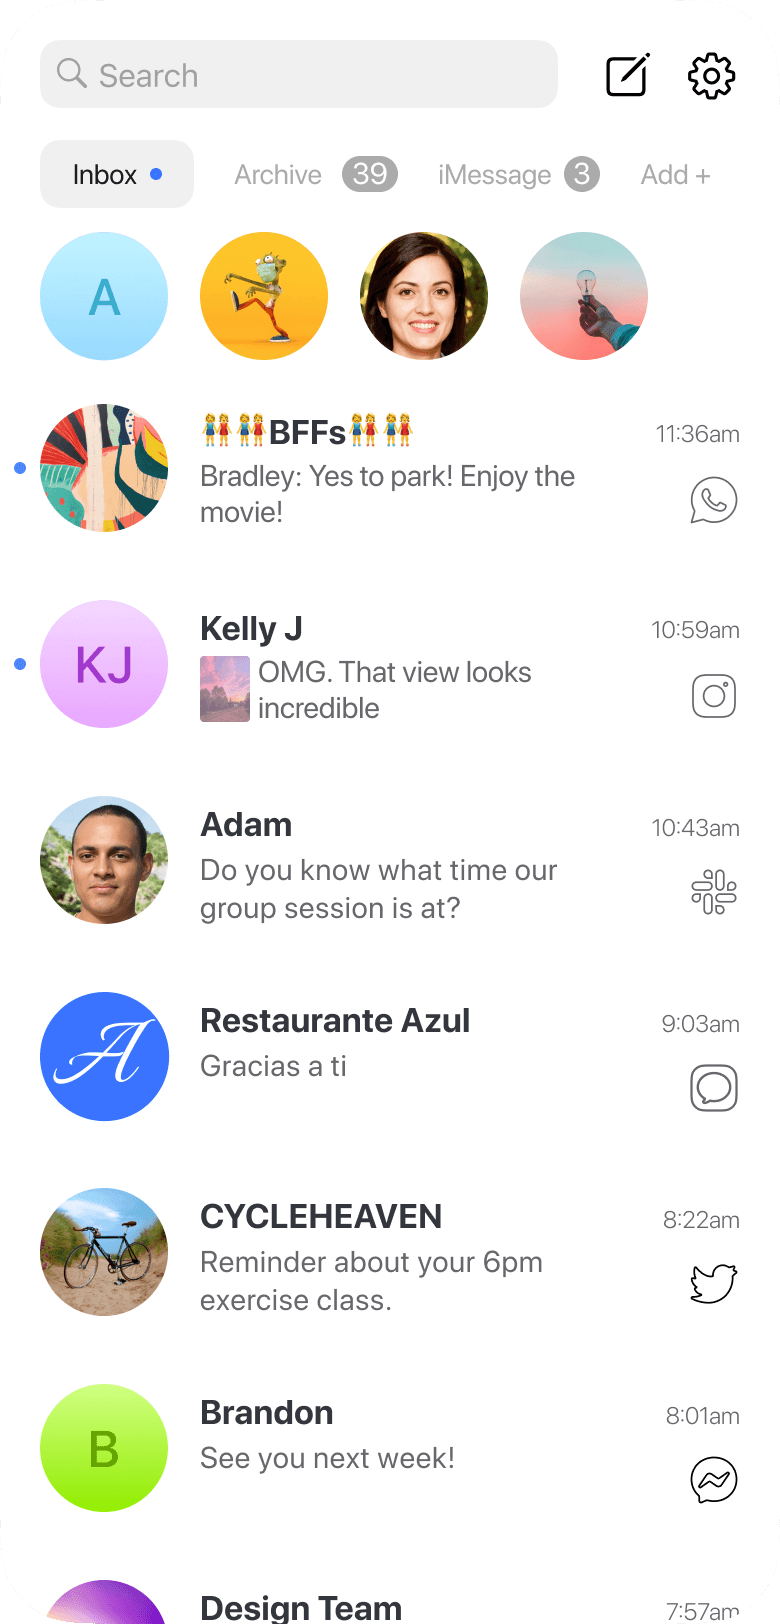
\includegraphics[width=0.3\textwidth]{images/beeper-mobile}}
\end{frame}

\begin{frame}{What is Beeper?}
    \textbf{Beeper allows you to consolidate messages from 15+ chat apps into a
        single inbox.}

    \pause
    \begin{itemize}
        \item Beeper is available on on macOS, Windows, Linux iPhone, iPad,
            Android and Chrome OS.
        \item Beeper is built on top of the Matrix protocol.
        \item Beeper encrypts all chats, including bridged chats, by
            default\footnote[frame]{We have to momentarily decrypt your chat
            messages to translate from the other network to Matrix, but we never
            log or store your unencrypted messages.}.
    \end{itemize}
\end{frame}

\begin{frame}{We are targeting individuals, not enterprises}
    \begin{center}
        \textbf{\Large We want to beat WhatsApp, not Slack.}
        \vspace{1cm}
        \pause

        \textbf{\large Our core competency is the 50th highest priority at the
        big tech companies.}

        Most chat networks are an afterthought within the ecosystem of a larger
        company. At Beeper, chat is all we care about.
    \end{center}
\end{frame}

\begin{frame}{How we make money}
    \textbf{We charge a flat \$10/month fee to use Beeper.} This fee allows
    users to connect as many chat networks as they want.
    \pause

    \textbf{No ads. No data mining.} We take advantage of Matrix's E2EE to add
    additional privacy guarantees.
    \pause

    \begin{center}
        \LARGE
        \textbf{The transaction is simple:\\ users pay us money for a service.}
    \end{center}
\end{frame}

\begin{frame}{Bridging to a glorious Matrix future}
    We see bridges as a way to onboard users into the Matrix ecosystem.

    Users can switch to a new app without losing a single conversation!
    \pause

    \vspace{1cm}
    \begin{center}
        \Large
        \textbf{We encourage our users to connect \textit{all} of their chat
        networks to Beeper.}
    \end{center}
\end{frame}

\section{What we've built}

\begin{frame}{Custom clients for desktop and mobile}
    We forked Element, and added custom features.
    \vspace{0.5cm}

    \centerline{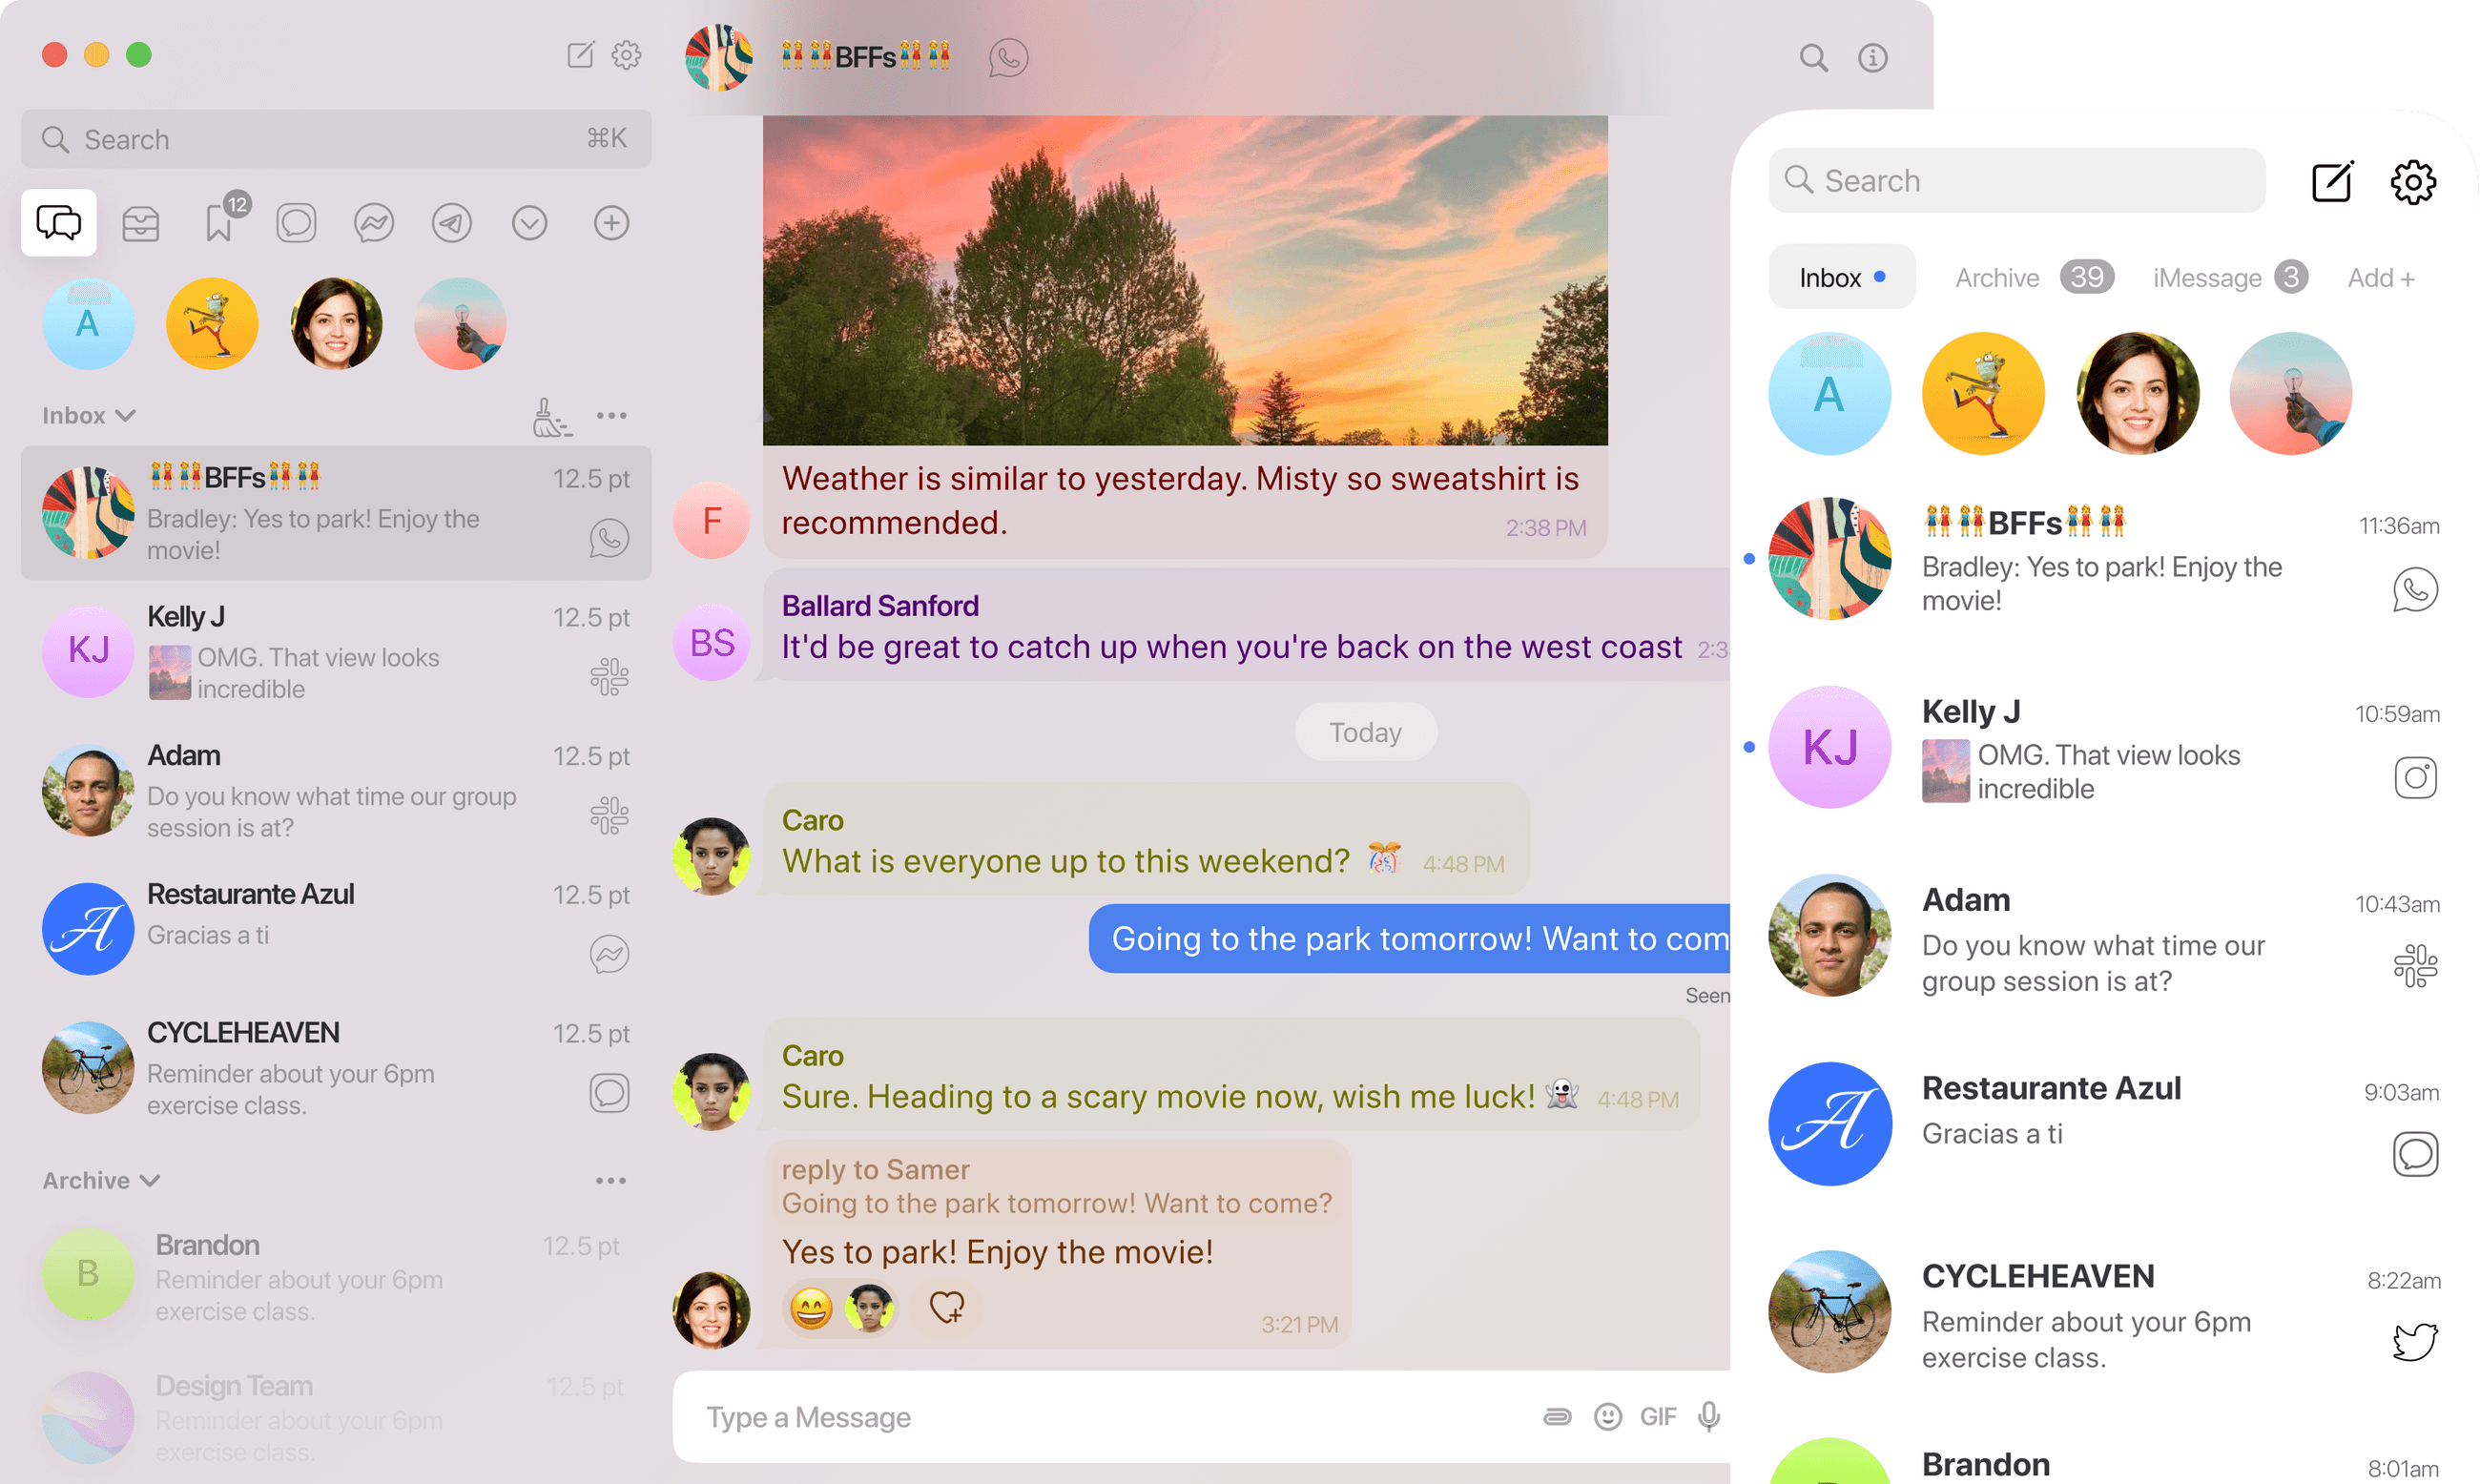
\includegraphics[width=\textwidth]{images/desktop-and-mobile}}
\end{frame}

\begin{frame}{Bridges, bridges, and more bridges!}
    We have built bridges to 10 networks:
    \begin{multicols}{2}
        \begin{itemize}
            \item iMessage
            \item WhatsApp
            \item Facebook Messenger
            \item SMS (Android)
            \item Telegram
            \item Signal
            \item LinkedIn
            \item Instagram
            \item Twitter
            \item Google Chat
        \end{itemize}
    \end{multicols}

    \pause
    We are actively developing new mautrix-based bridges to Discord and Slack.

    \pause
    You can also connect to IRC (via the Libera.chat bridge) and the rest of the
    Matrix federation.
\end{frame}

\begin{frame}{Easy chat network connection from clients}
    \centerline{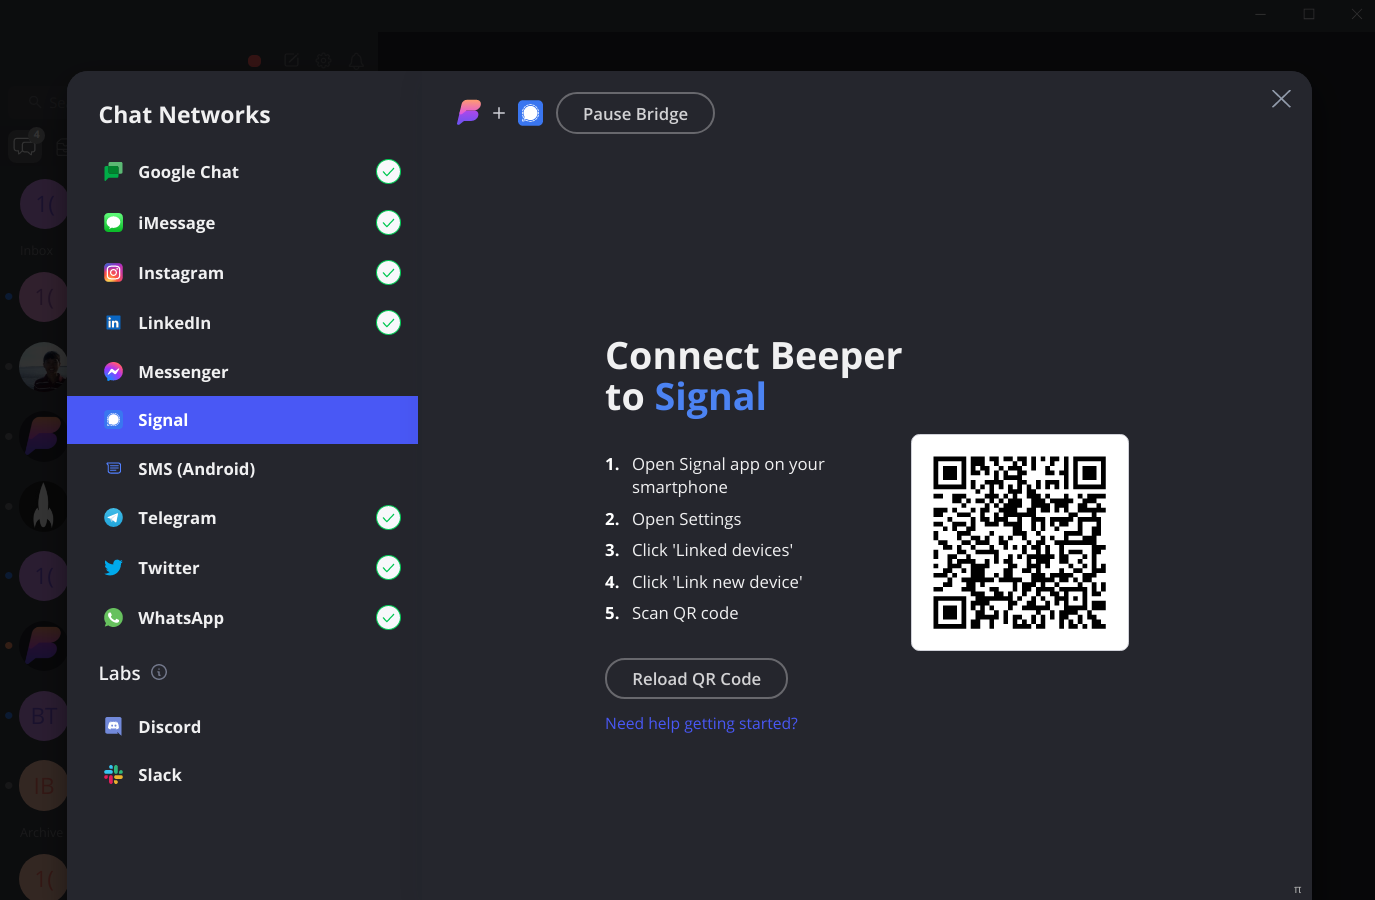
\includegraphics[width=0.9\textwidth]{images/chat-networks-dialog}}

    I'll demo this later!
\end{frame}

\begin{frame}{Chat inbox management tools}
    \begin{columns}
        \begin{column}{0.3\textwidth}
            \centerline{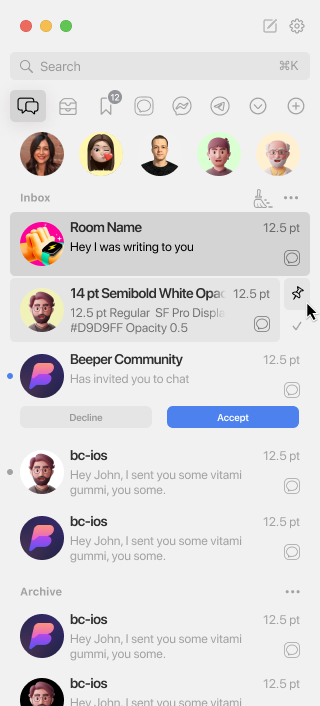
\includegraphics[width=\textwidth]{images/inbox-3.0}}
        \end{column}
        \begin{column}{0.7\textwidth}
            We've implemented lots of useful inbox management features such as:
            \begin{itemize}
                \item chat pinning
                \item chat archiving
                \item configurable auto-archive
                \item mark as read
                \item chat muting
                \item keyboard shortcuts
            \end{itemize}
        \end{column}
    \end{columns}
\end{frame}

\begin{frame}{Start new chat}
    \begin{columns}
        \begin{column}{0.6\textwidth}
            On some networks, you can start a new chat directly from Beeper.
            \vspace{1cm}

            You can also load your Google Contacts to get the correct names on
            your chats.
        \end{column}
        \begin{column}{0.4\textwidth}
            \centerline{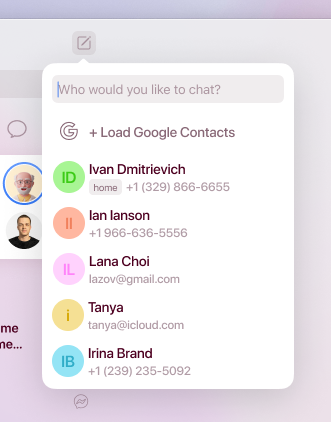
\includegraphics[width=\textwidth]{images/start-new-chat}}
        \end{column}
    \end{columns}
\end{frame}

\begin{frame}{Much, much, more!}
    \begin{multicols}{2}
        \begin{itemize}
            \item Message send status
            \item E2BE on all bridges
            \item Command bar (Ctrl+K)
            \item Scheduled messages
            \item Per-network spaces
            \item Universal search
        \end{itemize}
    \end{multicols}
\end{frame}

\begingroup
\def\insertframenumber{\relax}
\begin{frame}[standout]
    \Large
    Demo!
\end{frame}
\endgroup

\section{Current challenges}

\begin{frame}{Scaling: Problem}
    \textbf{Each user gets their own bridge for each network they connect.}

    That means we run a lot of bridges, and each bridge brings more traffic!
    \pause

    \begin{itemize}
        \item On average, each user brings \textbf{4716 puppeted users}.
        \item On average, each user and their puppets collectively account for
            \textbf{100k events}!
    \end{itemize}

    \pause
    None of the bridge traffic is federated, but Synapse is aggressively
    federated.
\end{frame}

\begin{frame}{Scaling: Solution}
    \begin{center}
        \textbf{We are sharding our homeserver based on bridged vs. unbridged
        traffic.} \\
        The new service for bridged traffic is called \textit{Hungryserv}.
    \end{center}
    \vspace{1cm}
    \pause

    By siphoning off unfederated bridge traffic to a different service, we allow
    Synapse to do what it does best: federate with other Matrix homeservers.
    \pause

    We can also optimize operations such as room deletion and infinite backfill.

    Because it's unfederated, we don't have to implement state resolution.
\end{frame}

\begin{frame}{The iOS app}
    Beeper's clients are forks of Element's clients. Having the Element
    codebase as a starting point has been hugely beneficial to us.
    \pause

    However, the iOS app needs some love.
    \vspace{1cm}
    \pause

    Element is currently working on Element X for iOS which uses the Rust SDK.

    We are taking a different approach: \textbf{rewriting the iOS app
    piece-by-piece and changing the architecture as necessary.}
\end{frame}

\section{What it's like to work at Beeper}

\begin{frame}{What I work on at Beeper}
    I am on the newly created \textit{Scaling} team.

    Our current objective is to prepare Beeper for rocket-ship growth.
    \vspace{0.5cm}
    \pause

    I was previously part of the \textit{Bridges} team. 

    Notable projects included:
    \begin{itemize}
        \item Writing the LinkedIn bridge
        \item Adding bridge status reporting and message send status
        \item Implementing massive stability improvements in the Signal bridge
        \item Implementing incremental infinite backfill in our WhatsApp and
            Facebook bridges
    \end{itemize}
\end{frame}

\begin{frame}{Weekly team rituals}
    \textbf{Demo Day:} Every Monday, we have a company-wide meeting where anyone
    on the team can present a demo of what they have been working on.
    \pause

    \textbf{Weekly Planning:} After demos, each team has a meeting to discuss
    what they are going to work on.
    \pause

    \textbf{Daily Standups:} On Tuesday to Friday, we have standups for each
    team.
    \pause

    \textbf{1:1s with Brad:} At least every other week, everyone has 1:1 with
    their boss.
\end{frame}

\begin{frame}{BRAD days: hacking to make Beeper a better company}
    Every third Friday, we have a Beeper Radical Awesomeness Day (BRAD).

    \begin{itemize}
        \item  BRAD is an optional day to build whatever you want to make Beeper
            a better company to work at.
        \item Some BRAD day projects have made it into clients such as scheduled
            messages.
        \item Other projects include internal tools such as bots, build
            automations, POCs, and more.
    \end{itemize}
\end{frame}

\begin{frame}{Team Retreats}
    About three times a year, we have a team retreat.

    \centerline{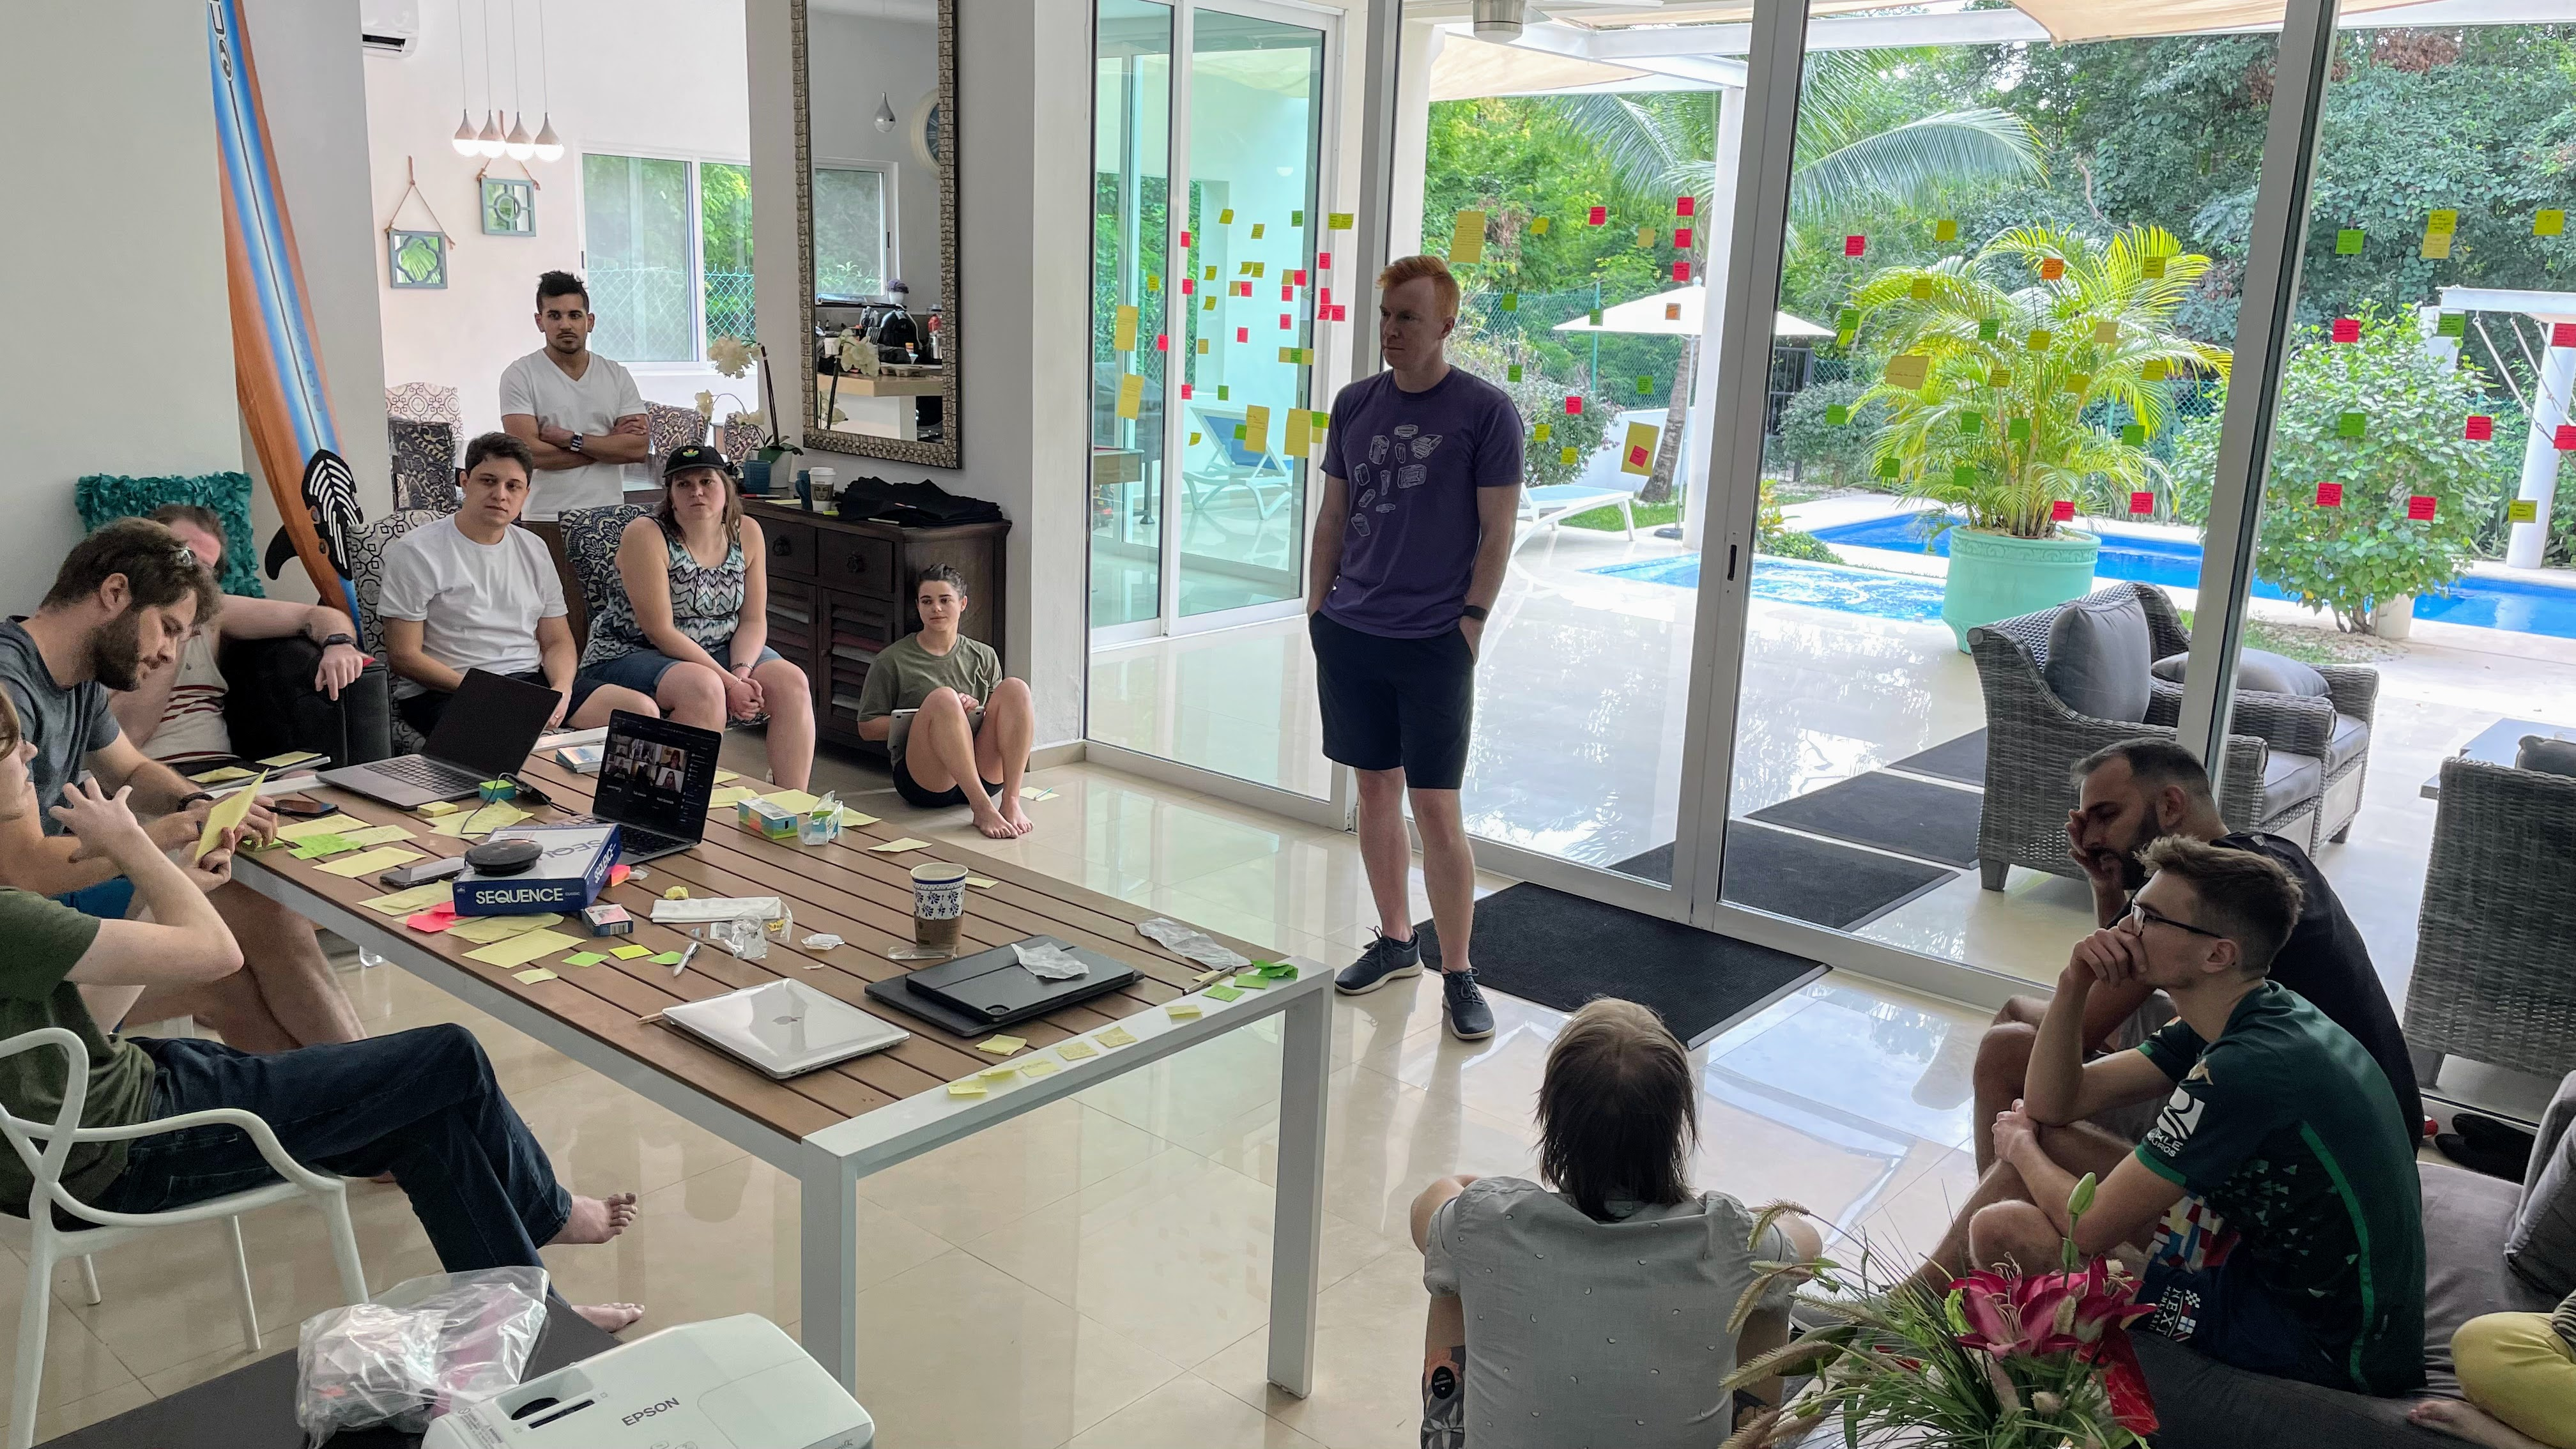
\includegraphics[width=\textwidth]{images/retro}}

    {
        You can read more about them on my blog at
        \href{https://sumnerevans.com/categories/work-retreats/}{\texttt{sumnerevans.com/categories/work-retreats}}.
    }
\end{frame}

\begingroup
\def\insertframenumber{\relax}
\begin{frame}[standout]
    \Huge
    Questions?
    \vspace{2em}

    {\large You can also reach me at \texttt{@sumner:nevarro.space}}
\end{frame}
\endgroup

\end{document}
% Local Variables:
% TeX-command-extra-options: "-shell-escape"
% End:
